\documentclass[12pt, a4paper, oneside]{ctexart}
\usepackage{amsmath, amsthm, amssymb, bm, color, graphicx, geometry, mathrsfs,extarrows, braket, booktabs, array, wrapfig, enumitem}
\usepackage[colorlinks,linkcolor=red,anchorcolor=blue,citecolor=blue,urlcolor=blue,menucolor=black]{hyperref}
%%%% 设置中文字体 %%%%
% fc-list -f "%{family}\n" :lang=zh >d:zhfont.txt 命令查看已有字体
\setCJKmainfont[
    BoldFont=方正黑体_GBK,  % 黑体
    ItalicFont=方正楷体_GBK,  % 楷体
    BoldItalicFont=方正粗楷简体,  % 粗楷体
    Mapping = fullwidth-stop  % 将中文句号“.”全部转化为英文句号“.”
]{方正书宋简体}  % !!! 注意在Windows中运行请改为“方正书宋简体.ttf” !!!
%%%% 设置英文字体 %%%%
\setmainfont{Minion Pro}
\setsansfont{Calibri}
\setmonofont{Consolas}

%%%% 设置行间距与页边距 %%%%
\linespread{1.4}
%\geometry{left=2.54cm,right=2.54cm,top=3.18cm,bottom=3.18cm}
\geometry{left=1.84cm,right=1.84cm,top=2.18cm,bottom=2.18cm}

%%%% 图片相对路径 %%%%
\graphicspath{{figures/}} % 当前目录下的figures文件夹, {../figures/}则是父目录的figures文件夹
\setlength{\abovecaptionskip}{-0.2cm}  % 缩紧图片标题与图片之间的距离
\setlength{\belowcaptionskip}{0pt} 

%%%% 缩小item,enumerate,description两行间间距 %%%%
\setenumerate[1]{itemsep=0pt,partopsep=0pt,parsep=\parskip,topsep=5pt}
\setitemize[1]{itemsep=0pt,partopsep=0pt,parsep=\parskip,topsep=5pt}
\setdescription{itemsep=0pt,partopsep=0pt,parsep=\parskip,topsep=5pt}

%%%% 自定义公式 %%%%
\everymath{\displaystyle} % 默认全部行间公式
\DeclareMathOperator*\uplim{\overline{lim}} % 定义上极限 \uplim_{}
\DeclareMathOperator*\lowlim{\underline{lim}} % 定义下极限 \lowlim_{}
\DeclareMathOperator*{\argmax}{arg\,max}  % 定义取最大值的参数 \argmax_{}
\DeclareMathOperator*{\argmin}{arg\,min}  % 定义取最小值的参数 \argmin_{}
\let\leq=\leqslant % 将全部leq变为leqslant
\let\geq=\geqslant % geq同理
\DeclareRobustCommand{\rchi}{{\mathpalette\irchi\relax}}
\newcommand{\irchi}[2]{\raisebox{\depth}{$#1\chi$}} % 使用\rchi将\chi居中

%%%% 自定义环境配置 %%%%
\newcounter{problem}  % 问题序号计数器
\newenvironment{problem}[1][]{\stepcounter{problem}\par\noindent\textbf{题目\arabic{problem}. #1}}{\smallskip\par}
\newenvironment{solution}[1][]{\par\noindent\textbf{#1解答. }}{\smallskip\par}  % 可带一个参数表示题号\begin{solution}{题号}
\newenvironment{note}{\par\noindent\textbf{注记. }}{\smallskip\par}
\newenvironment{remark}{\begin{enumerate}[label=\textbf{注\arabic*.}]}{\end{enumerate}}

%%%% 一些宏定义 %%%%
\def\bd{\boldsymbol}        % 加粗(向量) boldsymbol
\def\disp{\displaystyle}    % 使用行间公式 displaystyle(默认)
\def\weekto{\rightharpoonup}% 右半箭头
\def\tsty{\textstyle}       % 使用行内公式 textstyle
\def\sign{\text{sign}}      % sign function
\def\wtd{\widetilde}        % 宽波浪线 widetilde
\def\R{\mathbb{R}}          % Real number
\def\N{\mathbb{N}}          % Natural number
\def\Z{\mathbb{Z}}          % Integer number
\def\Q{\mathbb{Q}}          % Rational number
\def\C{\mathbb{C}}          % Complex number
\def\K{\mathbb{K}}          % Number Field
\def\P{\mathbb{P}}          % Polynomial
\def\E{\mathbb{E}}          % Exception
\def\d{\mathrm{d}}          % differential operator
\def\e{\mathrm{e}}          % Euler's number
\def\i{\mathrm{i}}          % imaginary number
\def\re{\mathrm{Re}}        % Real part
\def\im{\mathrm{Im}}        % Imaginary part
\def\res{\mathrm{Res}}      % Residue
\def\ker{\mathrm{Ker}}      % Kernel
\def\vspan{\mathrm{vspan}}  % Span  \span与latex内核代码冲突改为\vspan
\def\L{\mathcal{L}}         % Loss function
\def\O{\mathcal{O}}         % big O notation
\def\wdh{\widehat}          % 宽帽子 widehat
\def\ol{\overline}          % 上横线 overline
\def\ul{\underline}         % 下横线 underline
\def\add{\vspace{1ex}}      % 增加行间距
\def\del{\vspace{-1.5ex}}   % 减少行间距
\def\prob{\textrm{P}}       % Probability

%%%% 定理类环境的定义 %%%%
\newtheorem{theorem}{定理}

%%%% 基本信息 %%%%
\newcommand{\RQ}{\today} % 日期
\newcommand{\km}{随机过程} % 科目
\newcommand{\bj}{人工智能B2480} % 班级
\newcommand{\xm}{吴天阳} % 姓名
\newcommand{\xh}{4124136039} % 学号

\begin{document}

%\pagestyle{empty}
\pagestyle{plain}
\vspace*{-15ex}
\centerline{\begin{tabular}{*5{c}}
    \parbox[t]{0.25\linewidth}{\begin{center}\textbf{日期}\\ \large \textcolor{blue}{\RQ}\end{center}} 
    & \parbox[t]{0.2\linewidth}{\begin{center}\textbf{科目}\\ \large \textcolor{blue}{\km}\end{center}}
    & \parbox[t]{0.2\linewidth}{\begin{center}\textbf{班级}\\ \large \textcolor{blue}{\bj}\end{center}}
    & \parbox[t]{0.1\linewidth}{\begin{center}\textbf{姓名}\\ \large \textcolor{blue}{\xm}\end{center}}
    & \parbox[t]{0.15\linewidth}{\begin{center}\textbf{学号}\\ \large \textcolor{blue}{\xh}\end{center}} \\ \hline
\end{tabular}}
\begin{center}
    \zihao{3}\textbf{第12周作业\quad Markov链}
\end{center}\vspace{-0.2cm}
\begin{problem}
    \textbf{(P218 1.)}
    3个白球和3个黑球分布在两个坛子中,每个含有3个球。如果第一个坛子中有$i$个白球,
    我们就称此系统处在状态$i, i=0,1,2,3$。每次我们从坛子中取出一球,并将从第一个坛子中取出的球放到第二个坛子中,
    从第二个坛子取出的球放到第一个坛子中,以$X_n$记第$n$步后系统的状态。解释为什么$\{X_n,n\geqslant 0\}$是Markov链,并计算它的转移概率矩阵。
\end{problem}
\begin{solution}
    Markov性:每次交换操作仅和当前的坛子的状态决定,和历史中的坛子状态没有关系,因此满足Markov链性质。

    当系统处于状态$i$时,第一个坛子有$i$个白球$3-i$个黑球,\add
    第二个坛子有$3-i$个白球$i$个黑球,因此第一个坛子取出白球和黑球概率分别为$\frac{i}{3}$和$\frac{3-i}{3}$,第二个坛子同理。\add
    则当$i\in\{1,2\}$时,状态转移分以下三种情况
    \begin{itemize}
        \item 同时取出白球或黑球$P_{i,i} = \frac{2i(3-i)}{9}$;
        \item 第一和二个坛子分别取出白球和黑球$P_{i,i-1} = \frac{i^2}{9}$;
        \item 第一和二个坛子分别取出黑球和白球$P_{i,i+1} = \frac{(3-i)^2}{9}$.
    \end{itemize}
    而当$i\in\{0,3\}$时,仅能转移到相邻的状态上,综上,转移概率矩阵为
    \begin{equation*}
        P = \begin{bmatrix}
            0&1&0&0\\
            1/9&4/9&4/9&0\\
            0&4/9&4/9&1/9\\
            0&0&1&0
        \end{bmatrix}
    \end{equation*}
\end{solution}
\begin{problem}
    \textbf{P218 5.}
    一个状态为$0,1$或$2$的Markov链$\{X_n,n\geqslant 0\}$,它的转移概率矩阵为
    \begin{equation*}
        P = \begin{bmatrix}
            1/2&1/3&1/6\\
            0&1/3&2/3\\
            1/2&0&1/2
        \end{bmatrix}
    \end{equation*}
    如果$\prob(X_0=0)=\prob(X_0=1)=1/4$,求$\E[X_3]$.
\end{problem}
\begin{solution}
    由$C-K$方程可知,累计走$n$步的转移概率矩阵为
    \begin{equation*}
        P^3 = P^{(3)} = \begin{bmatrix}
        13/36 & 11/54 & 47/108 \\
        4/9 & 4/27 & 11/27 \\
        5/12 & 2/9 & 13/36
        \end{bmatrix}
    \end{equation*}
    则
    \begin{equation*}
        \E[X_3] = \sum_{j=0}^2\sum_{i=0}^2 \prob(X_0=i)P_{ij}^3\cdot j =
        \begin{bmatrix}
            1/4&1/4&1/2
        \end{bmatrix}P^3\begin{bmatrix}
            0\\1\\2
        \end{bmatrix} = \frac{53}{54}\approx 0.98148148
    \end{equation*}
\end{solution}
\begin{problem}\textbf{(P219 6.)}
    令两个状态的Markov链的转移概率矩阵为
    \begin{equation*}
        P = \begin{bmatrix}
            p&1-p\\1-p&p
        \end{bmatrix}
    \end{equation*}
    用数学归纳法证明
    \begin{equation*}
        P^{(n)} = \begin{bmatrix}
            \frac{1}{2}+\frac{1}{2}(2p-1)^n&\frac{1}{2}-\frac{1}{2}(2p-1)^n\\[1em]
            \frac{1}{2}-\frac{1}{2}(2p-1)^n&\frac{1}{2}+\frac{1}{2}(2p-1)^n
        \end{bmatrix}
    \end{equation*}
\end{problem}
\begin{proof}
    当$n=1$时,$P^{(n)} = \begin{bmatrix}
        \frac{1}{2}+\frac{1}{2}(2p-1)^1&\frac{1}{2}-\frac{1}{2}(2p-1)^1\\[1em]
        \frac{1}{2}-\frac{1}{2}(2p-1)^1&\frac{1}{2}+\frac{1}{2}(2p-1)^1
    \end{bmatrix} =
    \begin{bmatrix}
        p&1-p\\1-p&p
    \end{bmatrix}$成立。\add

    $\forall k\in\N^+$,只需证$P^{k+1} = P^{k}P$,令
    \begin{equation*}
        A = \begin{bmatrix}
        \frac{1}{2}+\frac{1}{2}(2p-1)^k&\frac{1}{2}-\frac{1}{2}(2p-1)^k\\[1em]
        \frac{1}{2}-\frac{1}{2}(2p-1)^k&\frac{1}{2}+\frac{1}{2}(2p-1)^k
    \end{bmatrix}
    \begin{bmatrix}
        p&1-p\\1-p&p
    \end{bmatrix}
    \end{equation*}
    则
    \begin{align*}
    A_{00} =&\ \left(\frac{1}{2}+\frac{1}{2}(2p-1)^k\right)p+\frac{1}{2}-\frac{1}{2}(2p-1)^k-\left(\frac{1}{2}-\frac{1}{2}(2p-1)^k\right)p\\
    =&\ (2p-1)^kp+\frac{1}{2}-\frac{1}{2}(2p-1)^k=\frac{1}{2}+\frac{1}{2}(2p-1)^{k+1}
    \end{align*}
    \begin{align*}
    A_{01} =&\ \frac{1}{2}+\frac{1}{2}(2p-1)^k-\left(\frac{1}{2}+\frac{1}{2}(2p-1)^k\right)p+\left(\frac{1}{2}-\frac{1}{2}(2p-1)^k\right)p\\
    =&\ \frac{1}{2}+\frac{1}{2}(2p-1)^k-(2p-1)^kp = \frac{1}{2}-\frac{1}{2}(2p-1)^{k+1}
    \end{align*}
    同理可知$A_{10}=A_{01}, A_{11}=A_{00}$,于是$P^kP = A = P^{k+1}$,由归纳法可知原命题成立。
\end{proof}
\begin{problem}\textbf{(P219 14.)}
    指定如下Markov链的类,确定它们是否都是暂态或常返态。
    \begin{equation*}
        P_1=\begin{bmatrix}
            0&1/2&1/2\\
            1/2&0&1/2\\
            1/2&1/2&0
        \end{bmatrix},\quad P_2=\begin{bmatrix}
            0&0&0&1\\
            0&0&0&1\\
            1/2&1/2&0&0\\
            0&0&1&0
        \end{bmatrix},
    \end{equation*}
    \begin{equation*}
        P_3=\begin{bmatrix}
            1/2&0&1/2&0&0\\
            1/4&1/2&1/4&0&0\\
            1/2&0&1/2&0&0\\
            0&0&0&1/2&1/2\\
            0&0&0&1/2&1/2
        \end{bmatrix},\quad P_4=\begin{bmatrix}
            1/4&3/4&0&0&0\\
            1/2&1/2&0&0&0\\
            0&0&1&0&0\\
            0&0&1/3&2/3&0\\
            1&0&0&0&0
        \end{bmatrix}.
    \end{equation*}
\end{problem}
\begin{solution}如下图所示,可知$P_1$中$\{1,2,3\}$为常返类,Markov链不可约;
    $P_2$中$\{1,2,3,4\}$为常返类,Markov链不可约;
    $P_3$中$\{1,3\},\{4,5\}$分别为常返类,$\{2\}$为暂态类;
    $P_4$中$\{1,2\},\{3\}$分别为常返类,$\{4\},\{5\}$为暂态类。
    \begin{figure}[htbp]
        \centering
        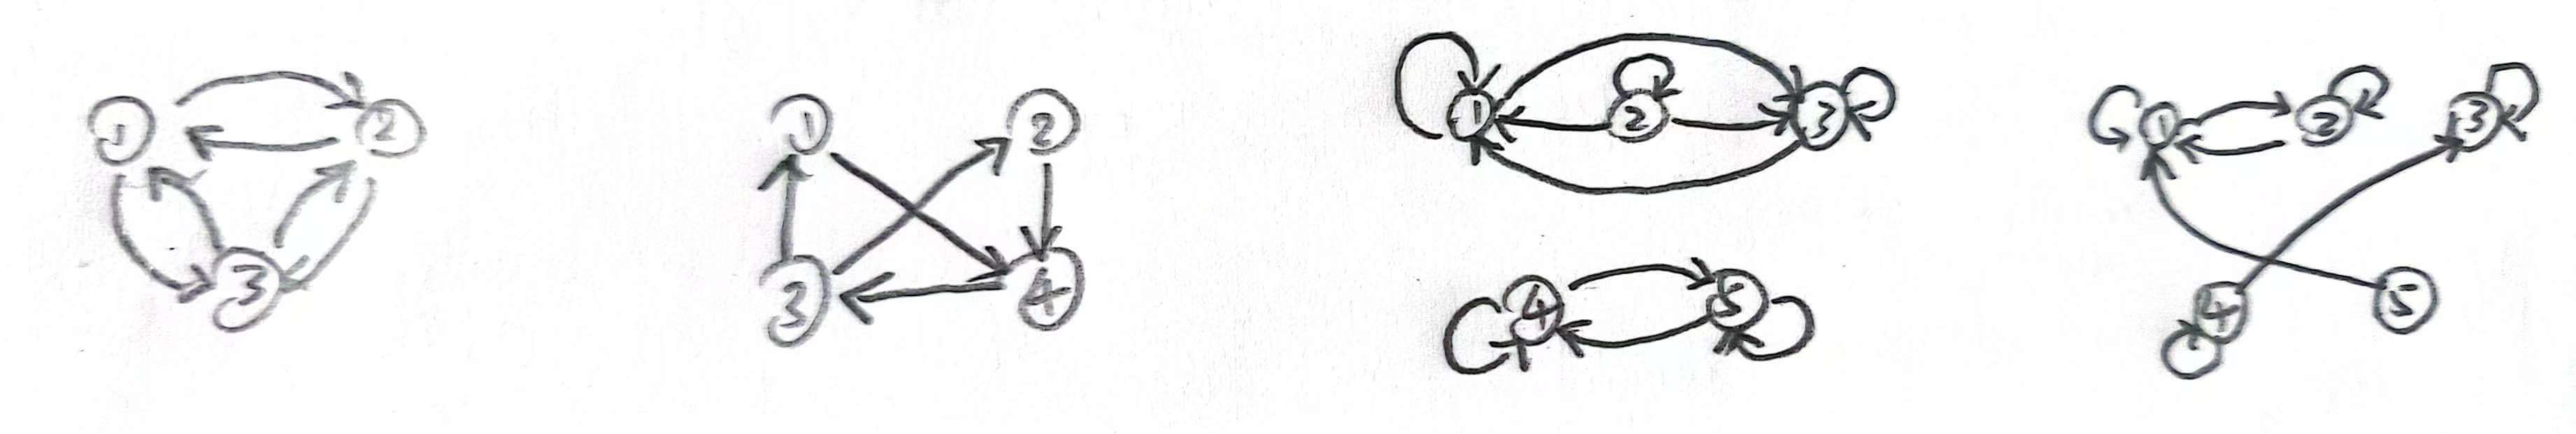
\includegraphics[width=\linewidth]{hw1_prob4.jpg}
        \caption{状态之间的可达关系图}
    \end{figure}
\end{solution}
\begin{problem}\textbf{(P220 16.)}
    证明若状态$i$为常返态,且状态$i$不与状态$j$互通,则$P_{ij}=0$。它说明一旦过程进入一个常返的状态类,
    它绝不会离开这个类。因为这个原因,一个常返类常指一个闭的类。
\end{problem}
\begin{proof}
    反设$P_{ij} > 0$,由于$i$为常返态,根据常返态性质有$j$也为常返态,因此$i$与$j$互通,矛盾,原命题成立。
\end{proof}
\begin{problem}
    \textbf{(P220 18.)}
    硬币$1$正面朝上的概率为$0.6$,而硬币$2$正面朝上的概率是$0.5$。一枚硬币连续地抛掷直到正面朝上,
    此时将这个硬币搁置一旁,我们开始抛掷另一枚。\\
    (a) 用硬币$1$抛掷的比例是多少?\\
    (b) 如果我们从抛掷硬币$1$开始,问第$5$次抛掷的是硬币$2$的概率是多少?
\end{problem}
\begin{solution}
    (a) 考虑两个状态的Markov链,状态$1$表示当前抛掷硬币$1$,状态$2$表示当前抛掷硬币$2$,每次抛出正面后换硬币,则转移概率矩阵为
    \begin{equation*}
        P=\begin{bmatrix}
            0.4&0.6\\
            0.5&0.5
        \end{bmatrix}
    \end{equation*}
    求解长程比例(平稳分布)$\pi\in\R^2$满足$\pi^T = \pi^T P, \pi_1+\pi_2 = 1$,解得$\pi_1=\frac{5}{11}, \pi_2=\frac{6}{11}$,
    则用硬币$1$抛掷的比例为$\frac{5}{11}$。

    (b) 求解$P$的特征值与特征向量:
    \begin{equation*}
        |P-\lambda I| = \left|\begin{matrix}
            0.4-\lambda&0.6\\
            0.5&0.5-\lambda
        \end{matrix}\right| = \lambda^2-\frac{9}{10}\lambda-\frac{1}{10} = 0
        \Rightarrow (\lambda-1)(10\lambda+1) = 0
    \end{equation*}
    特征值分别为$1, -0.1$,分别求出左特征向量
    \begin{align*}
        \bd{x}_1^T(P-I) =&\ 0 \Rightarrow \begin{cases}
            -0.6x_1+0.5x_2 = 0,\\
            0.6x_1-0.5x_2 = 0.
        \end{cases}\xrightarrow{\text{取特值}} \bd{x}_1=\left[\frac{5}{11},\frac{6}{11}\right]^T
    \end{align*}
    \begin{align*}
        \bd{x}_2^T(P-0.1I) =&\ 0 \Rightarrow \begin{cases}
            0.5x_1+0.5x_2 = 0,\\
            0.6x_1+0.6x_2 = 0.
        \end{cases}\xrightarrow{\text{取特值}} \bd{x}_2=\left[1,-1\right]^T\\
    \end{align*}
    初始状态分布为$\bd{v}_0 = [1,0]^T = \bd{x}_1+\frac{6}{11}\bd{x}_2$,则五次转移后的状态分布为
    \begin{equation*}
        \bd{v}_5^T = \bd{v}_0^TP^5 = \bd{x_1} + \frac{6}{11}\bd{x}_2\cdot0.1^5
    \end{equation*}
    可得到达状态$2$的概率为
    \begin{equation*}
        \frac{6}{11}+\frac{6}{11}(-1)0.1^5 = \frac{6}{11}(1-0.1^5)\approx \frac{6}{11}\approx 0.5454545
    \end{equation*}
\end{solution}
\begin{problem}\textbf{P220 20.}
    一个转移概率矩阵$P$称为双随机的,如果每一列的和为$1$,即对于一切的$j$,
    \begin{equation*}
        \sum_{i}P_{ij} = 1
    \end{equation*}
    如果这样的链是不可约和非周期的,并且由$M+1$个状态$0,1,\cdots,M$组成,证明长程比例为
    \begin{equation*}
        \pi_j = \frac{1}{M+1},\quad j=0,1,\cdots, M
    \end{equation*}
\end{problem}
\begin{proof}
    $\forall i, j\in\{0,1,\cdots, M\}$
    \begin{equation*}
        \sum_{i=0}^M\pi_iP_{ij} = \sum_{i=0}^M\left(\frac{1}{M+1}\right)P_{ij} = \frac{1}{M+1}\sum_{i=0}^MP_{ij}
        \xlongequal{P\text{每一列的和为}1}\frac{1}{M+1} = \pi_j
    \end{equation*}
    又由于Markov链是不可约且非周期的,根据Perron-Frobenius定理,存在唯一的长程比例$\pi_j$。
\end{proof}
\begin{problem}\textbf{P221 27.}
    $N$个总体中的任意一个个体在每个时段可能积极也可能消极。如果一个个体在某个时段积极,
    那么与所有其他个体独立,他在下一个时段也积极的概率为$\alpha$。类似地,如果一个个体在某个时段消极,
    那么与所有其他个体独立,他在下一个时段也消极的概率为$\beta$。令$X_n$表示在时段$n$积极的个体数。\\
    (a) 证明$\{X_n,n\geqslant 0\}$是Markov链;\\
    (b) 求$\E[X_n|X_0=i]$;\\
    (c) 推导转移概率的表达式;\\
    (d)求恰有$j$个个体积极的长程时间比例。
\end{problem}
\begin{solution}
    (a) 由于每个个体的状态转移仅依赖于当前的状态,并且与其他个体独立,即$X_{n+1}$仅依赖于$X_n$的状态,
    满足Markov性,因此$\{X_n,n\geqslant 0\}$是Markov链。

    (b) 由全期望公式可知
    \begin{align*}
        &\ \E[X_{n+1}|X_0=i] = \alpha\E[X_{n}|X_0=i] + (1-\beta)(N-\E[X_n|X_0=i])\\
        \text{(简记)}\Rightarrow&\ \E_{n+1} = (\alpha+\beta-1)\E_{n+1} + (1-\beta)N
    \end{align*}
    此为线性差分方程,解为齐次线性差分方程的通解和特解的和,其导出的齐次方程为$\E_{n+1}=(\alpha+\beta-1)\E_{n}$,特征根$\lambda = \alpha+\beta-1$,
    则齐次方程解为$C(\alpha+\beta-1)^n$,将$E^*$带入求特解
    \begin{equation*}
        \E^* = (\alpha+\beta-1)\E^* + (1-\beta)N\Rightarrow E^* = \frac{(1-\beta)N}{2-\alpha-\beta}
    \end{equation*}
    于是原线性差分方程解为$\E_n = \E^*+C(\alpha+\beta-1)^n$,带入初始条件$\E_0 = i$,可得$C = i - \E^*$。
    
    综上
    \begin{equation*}
        \E[X_n|X_0=i] = \E^*+(i-\E^*)(\alpha+\beta-1)^n,\quad\text{其中}\ \E^* = \frac{(1-\beta)N}{2-\alpha-\beta}
    \end{equation*}

    (c) $\forall i, j\in\{0,1,\cdots,N\}$,\add $\forall k\leqslant\min\{i,j\}$表示连续两个状态保持积极的个体数,则从状态$i$到状态$j$的概率转移存在两种情况:
    $k$个积极个体保持积极,概率为$\binom{i}{k}\alpha^k(1-\alpha)^{i-k}$;$j-k$个消极个体变为积极个体,概率为
    $\binom{N-i}{j-k}\beta^{j-k}(1-\beta)^{N-i-(j-k)}$
    
    综上,转移概率表达式为
    \begin{equation*}
        P_{ij} = \sum_{k=\max\{0,i+j-N\}}^{\min\{i,j\}}\binom{i}{k}\alpha^k(1-\alpha)^{i-k}\binom{N-i}{j-k}\beta^{j-k}(1-\beta)^{N-i-(j-k)}
    \end{equation*}

    (d) 由于每个个体独立,且在两个状态中进行转移,假设平稳分布为二项分布,在平稳分布下处于积极的概率为$p$,则
    \begin{equation*}
        p = \alpha p+(1-\beta)(1-p)\Rightarrow p = \frac{1-\beta}{2-\alpha-\beta}
    \end{equation*}
    可得平稳分布为
    \begin{equation*}
        \pi_j = \binom{N}{j}\left(\frac{1-\beta}{2-\alpha-\beta}\right)^j\left(\frac{1-\alpha}{2-\alpha-\beta}\right)^{N-j}
    \end{equation*}
\end{solution}
\begin{problem}\textbf{P222 30.}
    在公路上,每$4$辆货车中有$3$辆后面跟着一辆轿车,而每$5$辆轿车中只有一辆后面跟着一辆货车。
    行驶在公路上的车辆中货车的比例是多少?
\end{problem}
\begin{solution}
    将该问题视为Markov过程,$X_n$表示第$n$辆车的车型,其中状态$1$表示当前为货车,状态$2$表示当前为轿车,则转移概率矩阵为
    \begin{equation*}
        P = \begin{bmatrix}
            1/4&3/4\\
            1/5&4/5
        \end{bmatrix}
    \end{equation*}
    求解长程比例$\pi\in\R^2$满足$\pi^T=\pi^TP, \pi_1+\pi_2=1$,解得$\pi_1=\frac{4}{19}$,故货车出现的比例为$4:19$。
\end{solution}
\end{document}
